%%%%%%%%%%%%%%%%%%%%%%%%%%%%%%%%%%%%%%%%%
% NIWeek 2014 Poster by T. Reveyrand
% www.microwave.fr
% http://www.microwave.fr/LaTeX.html
% ---------------------------------------
% 
% Original template created by:
% Brian Amberg (baposter@brian-amberg.de)
%
% This template has been downloaded from:
% http://www.LaTeXTemplates.com
%
% License:
% CC BY-NC-SA 3.0 (http://creativecommons.org/licenses/by-nc-sa/3.0/)
%
%%%%%%%%%%%%%%%%%%%%%%%%%%%%%%%%%%%%%%%%%

%----------------------------------------------------------------------------------------
%	PACKAGES AND OTHER DOCUMENT CONFIGURATIONS
%----------------------------------------------------------------------------------------

\documentclass[a0paper,portrait]{baposter}
\usepackage{graphicx}
\usepackage[font=small,labelfont=bf]{caption} % Required for specifying captions to tables and figures
\usepackage{booktabs} % Horizontal rules in tables
\usepackage{relsize} % Used for making text smaller in some places

\usepackage{amsmath,amsfonts,amssymb,amsthm} % Math packages
\usepackage{eqparbox}

\usepackage{textcomp}
\usepackage[
backend=biber,
style=alphabetic,
citestyle=numeric
]{biblatex}

\graphicspath{{../Figures/}} % Directory in which figures are stored

 \definecolor{bordercol}{RGB}{40,40,40} % Border color of content boxes
 \definecolor{headercol1}{RGB}{186,215,230} % Background color for the header in the content boxes (left side)
 \definecolor{headercol2}{RGB}{120,120,120} % Background color for the header in the content boxes (right side)
 \definecolor{headerfontcol}{RGB}{0,0,0} % Text color for the header text in the content boxes
 \definecolor{boxcolor}{RGB}{210,235,250} % Background color for the content in the content boxes


\begin{document}

\background{ % Set the background to an image (background.pdf)
\begin{tikzpicture}[remember picture,overlay]
\draw (current page.north west)+(-2em,2em) node[anchor=north west]
{\includegraphics[height=1.1\textheight]{background}};
\end{tikzpicture}
}
\definecolor{BGcolour}{RGB}{200,200,200}
\begin{poster}{
grid=false,
borderColor=bordercol, % Border color of content boxes
headerColorOne=headercol1, % Background color for the header in the content boxes (left side)
headerColorTwo=headercol2, % Background color for the header in the content boxes (right side)
headerFontColor=headerfontcol, % Text color for the header text in the content boxes
boxColorOne=boxcolor, % Background color for the content in the content boxes
headershape=roundedright, % Specify the rounded corner in the content box headers
headerfont=\Large\sf\bf, % Font modifiers for the text in the content box headers
textborder=rectangle,
%background=user,
bgColorOne=BGcolour, % declare background colour
background=plain,
headerborder=open, % Change to closed for a line under the content box headers
boxshade=plain
}

%
%----------------------------------------------------------------------------------------
%	TITLE AND AUTHOR NAME
%----------------------------------------------------------------------------------------
%
{ \bf  \huge {Traffic Sign Detection in Colour Images} } % Poster title
{\vspace{0.3em} \smaller Marvin Klaus$^1$, Daniela Schacherer$^2$  \\  % Author names
  
\smaller $^1$\it {Heidelberg University, M.Sc. Applied Computer Science} \\ $^2$\it{Heidelberg University, M.Sc. Applied Computer Science} \\ % Author email addresses  
  
 } % Author email addresses
%{\includegraphics[scale=0.45]{NI.jpg}} % University/lab logo

%----------------------------------------------------------------------------------------
%	INTRODUCTION
%----------------------------------------------------------------------------------------
\headerbox{Problem Definition}{name=introduction,column=0,row=0, span=3}{
Our project compares two state-of-the art approaches towards the detection of traffic signs in color images. The first approach uses a linear classifier, more precisely a support vector machine (SVM), based on Histogram of oriented gradients (HOG) features. The second approach employs a region based convolutional neural network (R-CNN). Our training set was made available by the University of Bochum in the context of a traffic sign detection competition in 2013 \cite{Houben-IJCNN-2013}. It comprises 900 images (1360
$\times$ 800 pixels) containing 1206 traffic signs. In addition, the image sections containing only the traffic signs and a CSV file containing ground truth information (location
of the traffic signs within the images) are provided.

\begin{center}
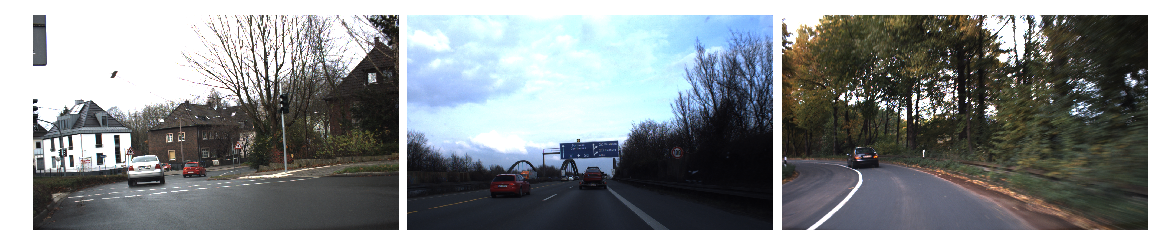
\includegraphics[width=0.6\textwidth]{ex_imgs_small.png}
\end{center}

}
 



%----------------------------------------------------------------------------------------
%	OTHER INSTRUMENTATION
%----------------------------------------------------------------------------------------
\headerbox{Approach 1: SVM based on HOG features}{name=instruments,span=2,column=0,row=1, below=introduction} % To reduce this block to 1 column width, remove 'span=2'
{
\textbf{Data Preprocessing}
\begin{itemize}
	\setlength\itemsep{0em}
	\item Preparation of positive image patches ($30 \times 30$ pixels) showing traffic signs.
	\item Preparation of negative image patches ($30 \times 30$ pixels) showing something that is not a sign. 
\end{itemize}

\textbf{Feature extraction}
\begin{itemize}
	\setlength\itemsep{0em}
	\item Extraction of HOG features from the positive and negative image patches using a HOG implementation from scikit \cite{scikithog}.
\end{itemize}


\begin{minipage}{0.48\textwidth}
\centering
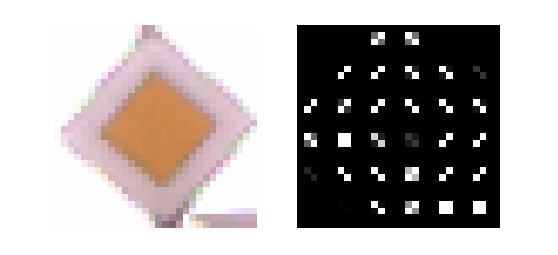
\includegraphics[width=0.7\linewidth]{hog_pos2_small.png}
\end{minipage}
\hfill
\begin{minipage}{0.48\textwidth}
\centering
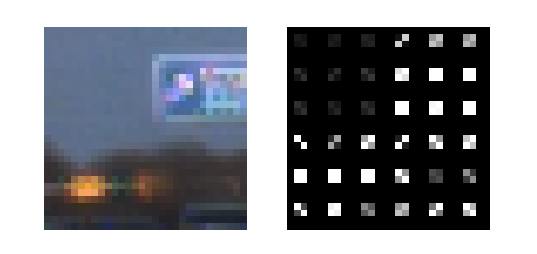
\includegraphics[width=0.7\linewidth]{hog_neg_small.png}
\end{minipage}


\textbf{Training}
\begin{itemize}
	\setlength\itemsep{0em}
	\item Fit the SVM to the prepared training data.
	\item Hard negative mining: apply the trained SVM to some of the training images - obtained with a sliding window of $30 \times 30$ pixels size and a step size of $10$ pixels at different scales. Each falsely detected patch is taken and explicitly added as a negative example to the training set.
	\item Fit the SVM using the enlarged training data.
\end{itemize}

\textbf{Detection of traffic signs in an image}
\begin{itemize}
	\setlength\itemsep{0em}
	\item Slide a window of $30 \times 30$ pixels size with a predefined step size (here: $5$ pixels) across the image at different scales and obtain a prediction for every image section from the SVM.
\end{itemize}

}




%----------------------------------------------------------------------------------------
%	MIXER vs. SAMPLERS
%----------------------------------------------------------------------------------------
%\headerbox{Receiver: Mixer vs. Sampler}{name=receiver,span=2,column=1,row=1, below=instruments}{
%\begin{center}
%\includegraphics[width=1\linewidth]{RECEIVER.pdf}
%\end{center}
%}


%----------------------------------------------------------------------------------------
%	MEASUREMENT SETUP
%----------------------------------------------------------------------------------------
\headerbox{Approach 2: R-CNN}{name=application,span=2,column=0,below=instruments}{ 
\textbf{Data Preprocessing}

\begin{minipage}{0.3\textwidth}
\centering
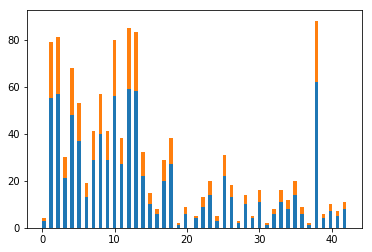
\includegraphics[width=1\linewidth]{data_hist}
\end{minipage}
\hfill
\begin{minipage}{0.65\textwidth}
\centering
\begin{itemize}
\item Create negative image patches by taking samples from traffic scenes without signs
\item Create train and test dataloader with following partition
\end{itemize}
\end{minipage}


\textbf{Network}
\begin{itemize}
\item Loss function: Cross Entropy Loss
\item Optimizer: Adam
\end{itemize}

}



%----------------------------------------------------------------------------------------
%	CONCLUSION
%----------------------------------------------------------------------------------------
\headerbox{Results SVM}{name=conclusion,column=2,below=introduction,span=1}{
\textbf{Performance Measure}: Each predicted bounding box $P$ is compared against every ground-truth $G$ using the Jaccard similarity (intersection over union): 
\begin{align*}
	S(P,G) = \frac{|P \cap G|}{|P \cup G|}
\end{align*}
When $S \geq 0.6$, the ground truth sign is considered as detected. Finally we record the fraction of detected ground truth signs in all images.\\

\begin{minipage}{\textwidth}
\centering
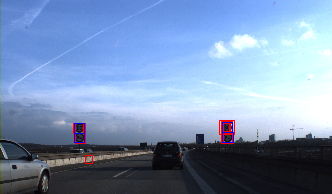
\includegraphics[width=0.7\linewidth]{test144_wb_predboxes2.png}
\end{minipage}

\textbf{Result}: The amount of correctly found traffic signs on 30 images from the train respectively test set obtained with and without HNM is shown in the following table. 

\centering
\small
\begin{tabular}{ l | r r }
  &  train acc & test acc \\ \toprule
  w/o HNM & 93.05 \% & 89.17 \% \\
  w HNM & 85.56 \% & 79.17 \% \\
\end{tabular}

}


%----------------------------------------------------------------------------------------
%	CALIBRATION
%----------------------------------------------------------------------------------------
\headerbox{Results R-CNN}{name=calibration,column=2,below=conclusion}{
\begin{minipage}{\textwidth}
\centering
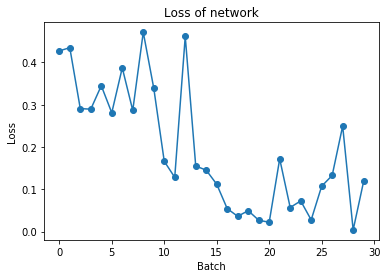
\includegraphics[width=0.75\linewidth]{loss}
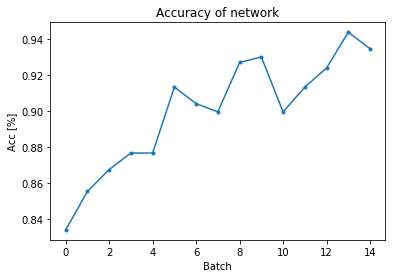
\includegraphics[width=0.75\linewidth]{acc}
\end{minipage}

\begin{itemize}
\item Selective Search to find interesting regions
	\begin{itemize}
	\item parameter: scale=300 and sigma=0.8
	\end{itemize}
\item Run network with every region to get signs
\item Same measurement as in SVM approach to find positive results
\end{itemize}

}


\headerbox{Comparison}{name=comparison,span=2,column=0,below=application}{ 
\textbf{Comparison}

The network of course is much faster when it comes to classify if something is a traffic sign or not. The downside is that the selective search algorithm takes much time to define interesting regions.\\
From accuracy perspective ...

}
%----------------------------------------------------------------------------------------
%	REFERENCES
%----------------------------------------------------------------------------------------

%\headerbox{References}{name=references,column=2,below=application}{

%\smaller % Reduce the font size in this block
%\renewcommand{\section}[2]{\vskip 0.05em} % Get rid of the default "References" section title
%\nocite{*} % Insert publications even if they are not cited in the poster

%\bibliographystyle{unsrt}
%\bibliographystyle{IEEEtran}
%\bibliography{biblio} % Use biblio.bib as the bibliography file
%}


%----------------------------------------------------------------------------------------
%	ACKNOWLEDGEMENTS
%----------------------------------------------------------------------------------------

%\headerbox{Acknowledgements}{name=acknowledgements,column=0,below=conclusion, above=bottom,span=3}{
%\smaller 
%This work is funded by National Instruments (Dr. Truchard) through a charitable donation. We would like to acknowledge DARPA (Dr. Greene) and ONR (Dr. Maki) for funding the initial part of this work under grant N00014-11-1-0931. \hfill \tiny \textit{Poster downloaded from} \textbf{www.microwave.fr}
%} 


\end{poster}

\end{document}